\documentclass[tikz]{standalone}

\usepackage{amsmath}
\usepackage{pgfplots}
\pgfplotsset{compat=1.16}
\pgfplotsset{
    no markers,
    axis lines=middle,
    xtick={\empty},
    ytick={\empty},
    every axis/.style={
        scale only axis,
        unit vector ratio*=1 1 1,
    },
    every axis plot/.append style={ultra thick},
    xlabel style={at={(ticklabel* cs:1)}, anchor=north west},
    ylabel style={at={(ticklabel* cs:1)}, anchor=east},
}


\newcommand\I[1]{\ensuremath{I_{\text{#1}}}}
\newcommand\V[1]{\ensuremath{V_{\text{#1}}}}

\def\vu{\V{u}}
\def\vbc{\V{BC}}
\def\vbe{\V{BE}}
\def\vce{\V{CE}}
\def\vi{\V{i}}
\def\vh{\V{H}}
\def\vl{\V{L}}
\def\vgg{\ensuremath{V_\gamma}}
\newcommand\vcesat{\ensuremath{V_{\text{CE}_{\text{SAT}}}}}

\def\vilmax{\ensuremath{{\V{IL}}_\text{MAX}}}
\def\vihmin{\ensuremath{{\V{IH}}_\text{MIN}}}
\def\nm{\ensuremath{{N}_\text{M}}}
\def\ls{\ensuremath{L_S}}
\def\vtl{\V{TL}}
\def\vohmin{\ensuremath{V_{\text{OH}_\text{MIN}}}}
\def\volmax{\ensuremath{V_{\text{OL}_\text{MAX}}}}
\def\nml{\ensuremath{N_\text{ML}}}
\def\nmh{\ensuremath{N_\text{MH}}}


\def\k{2}
\def\a{-1}
\def\n{0.05}
\def\A{3.2}
\def\int{1.8}

\begin{document}
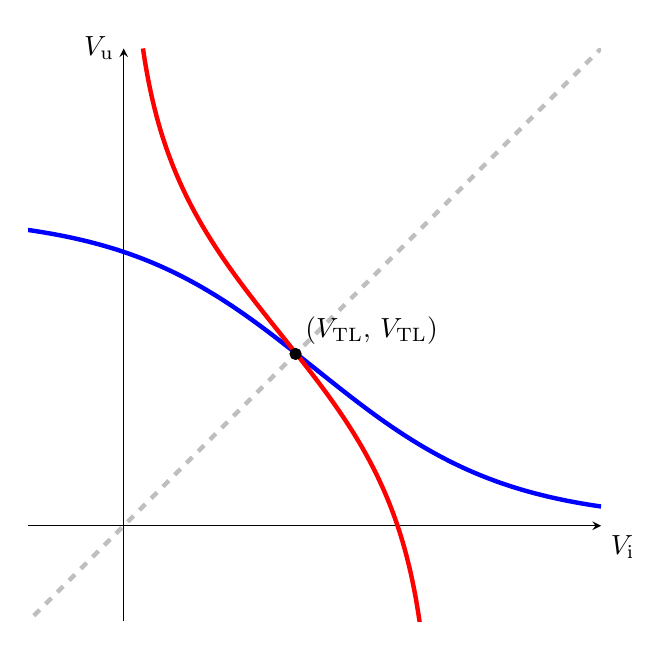
\begin{tikzpicture}
    \begin{axis}[xlabel=\vi, ylabel=\vu, ymin=-1, ymax=5, xmin=-1, xmax=5]
        \addplot[samples=200, color=blue]{
                \A * ((e^(\a*x + \k))/( 1 + e^(\a * x + \k))) + \n
            };
        \addplot[samples=200, color=red](
            \A * ((e^(\a*x + \k))/( 1 + e^(\a * x + \k))) + \n
            , x);
        \addplot[dashed, lightgray]{x};

        \filldraw[black]
            (\int, \int) circle(2pt) node[anchor=south west]{(\vtl, \vtl)}
            ;
    \end{axis}
\end{tikzpicture}
\end{document}
